\documentclass{article}
\usepackage[utf8]{inputenc}
\usepackage[OT2]{fontenc}
\usepackage[serbianc, serbian]{babel}
\usepackage{hyperref}
\usepackage{graphicx}
\usepackage{minted}
\usepackage{xcolor} % to access the named colour LightGray
\definecolor{LightGray}{gray}{0.9}

\usepackage{float}

\title{Izveshtaj primene alata za verifikaciju nad bibliotekom za detekciju lica}
\author{Marija Eric1 \\ 
$marija.eric@matf.bg.ac.rs$}

\date{Januar 2023}


\begin{document}

\maketitle
\renewcommand{\abstractname}{Sazhetak}
\renewcommand*\contentsname{Sadrzhaj}



\begin{abstract}
Projekat na kome je izvrshena analiza je biblioteka za detekciju lica, napisana u $C++$. Biblioteka je otvorenog koda i mozhe se pronac1i na narednom \href{https://github.com/ShiqiYu/libfacedetection}{linku}. 

\end{abstract}
\tableofcontents
\newpage

\section{Verifikacija softvera}
\subsection{Dinamichka analiza}
\subsubsection{$Gcov$}

Prikazana je pokrivenost za ispravno pokretanja primera upotrebe.

\begin{figure}[H]
    \centering
    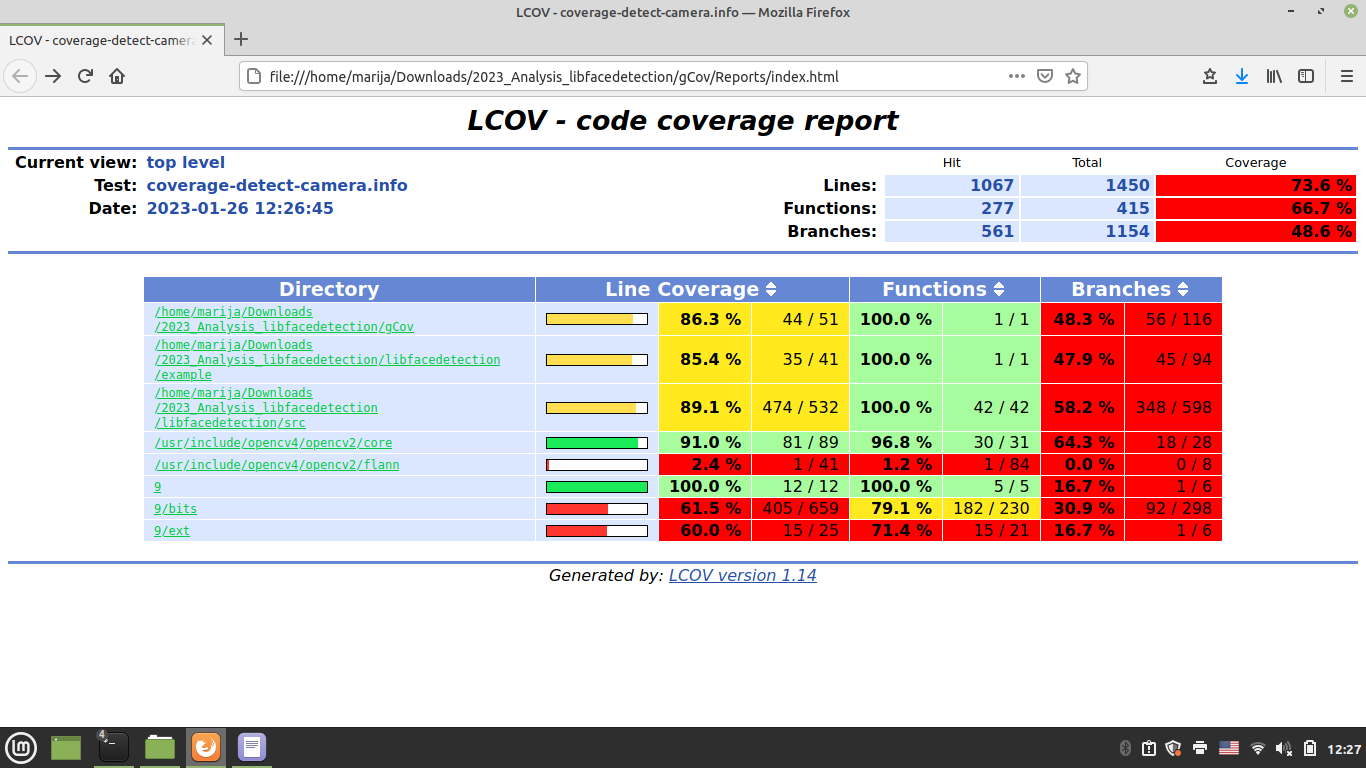
\includegraphics[width=12cm]{img/gcov/gcovCoverageDetect.png}
    \caption{Pokrivenost koda }
    \label{covd:gcov}
\end{figure}

%Vidimo da je velika pokrivenost svih datoteka, osim 9....
%U njima se nalaze pokretanja vezana za math i slichne biblioteke, i %sasvim je u redu da pokrivenost ne bude velika...

%Detaljnija pokrivenost za pokrivenost biblioteke, bas pokriveno, %koriste se sve funkcije definisane u biblioteci.

\begin{figure}[H]
    \centering
    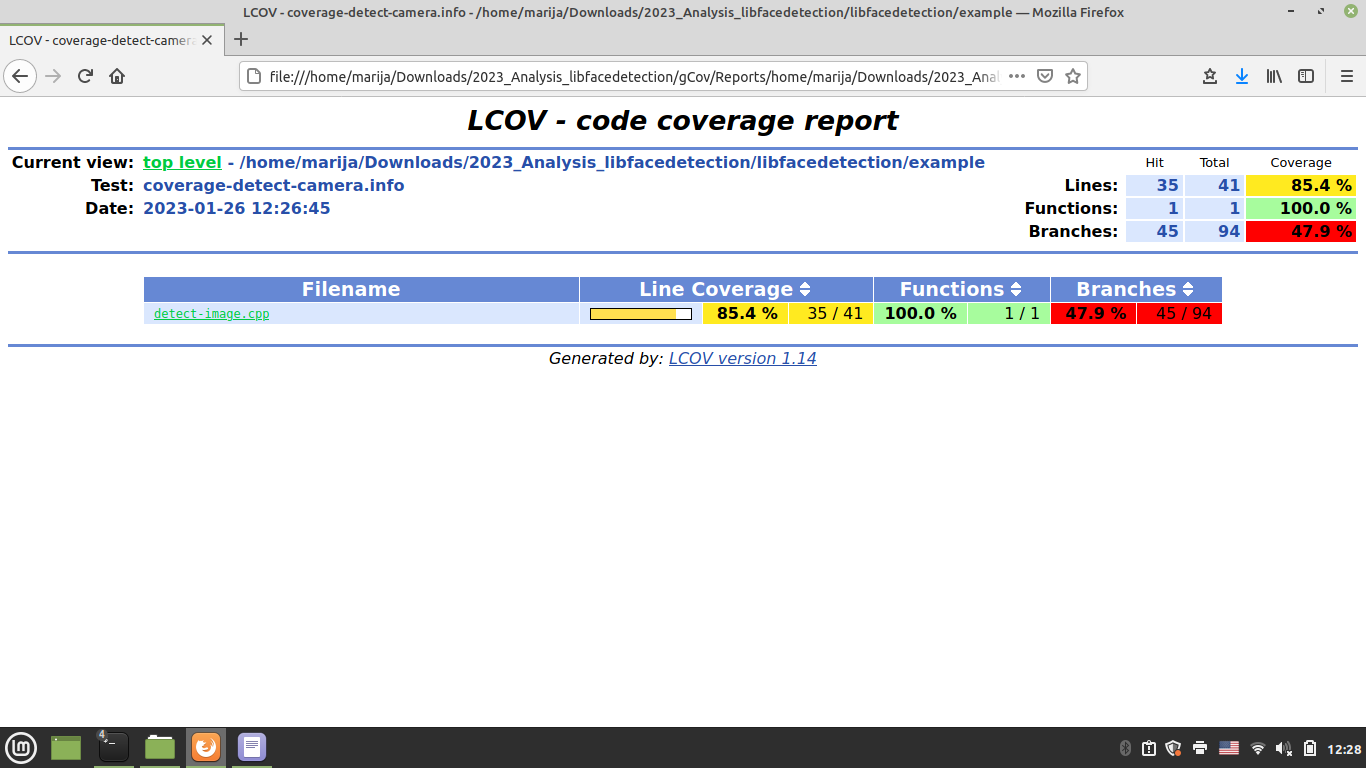
\includegraphics[width=12cm]{img/gcov/gcovDI.png}
    \caption{Pokrivenost koda pokretanjem detect image}
    \label{di:gcov}
\end{figure}
\begin{figure}[H]
    \centering
    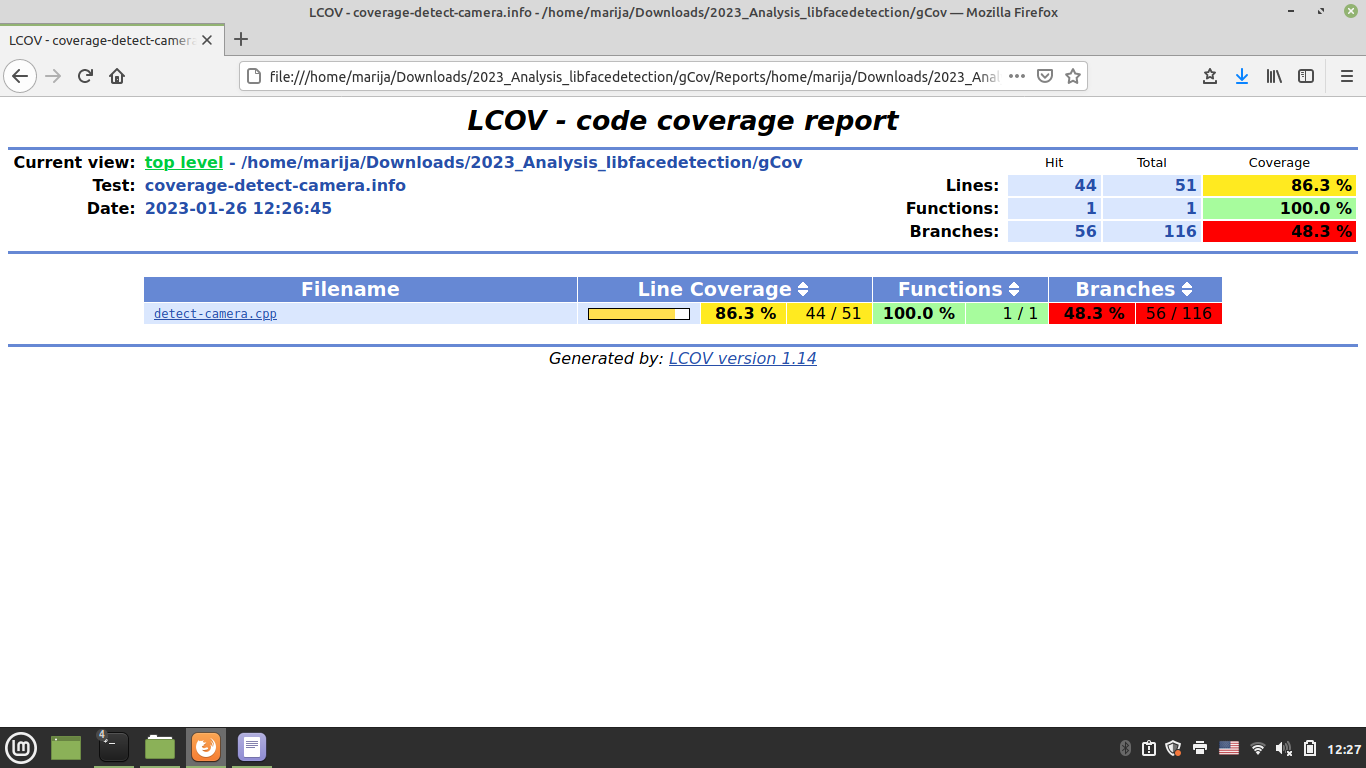
\includegraphics[width=12cm]{img/gcov/gcovDC.png}
    \caption{Pokrivenost koda detect camera}
    \label{dc:gcov}
\end{figure}
\begin{figure}[H]
    \centering
    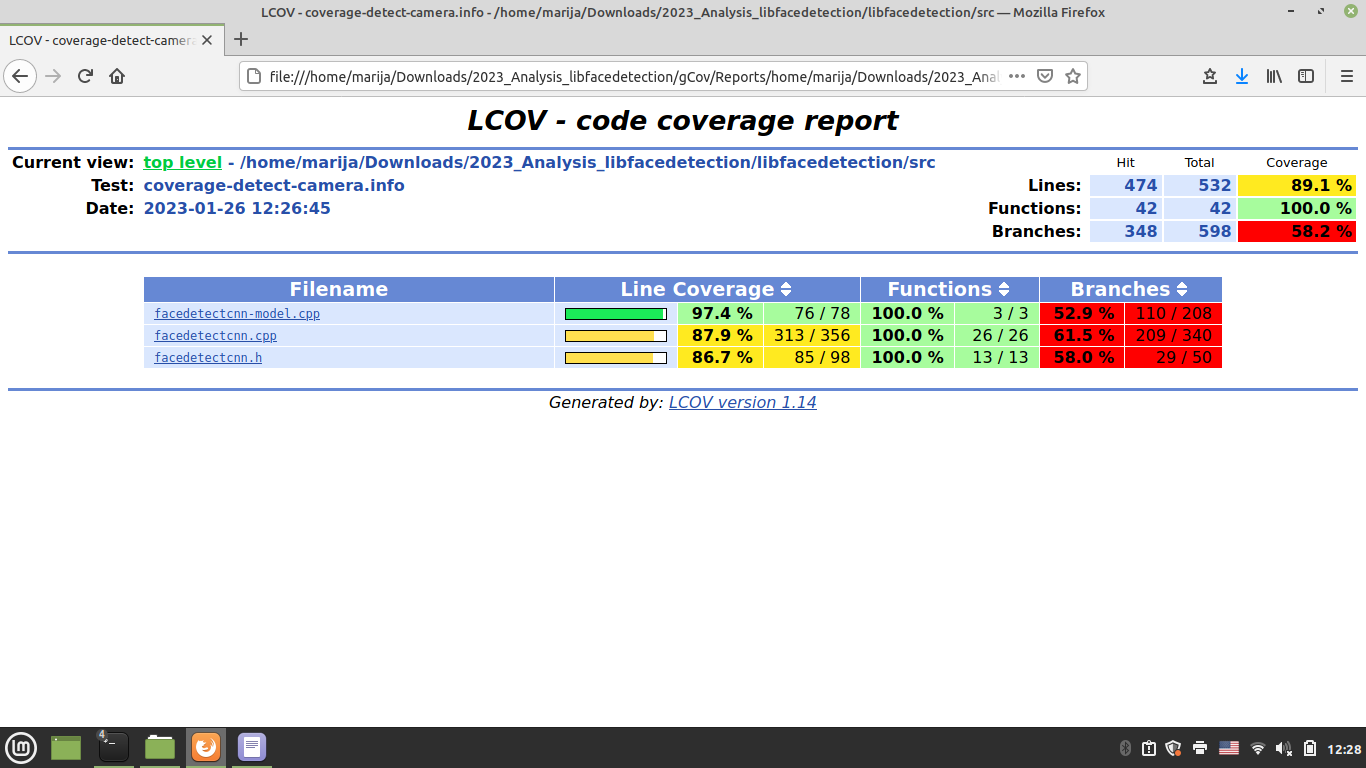
\includegraphics[width=12cm]{img/gcov/gcovSRC.png}
    \caption{Pokrivenost koda biblioteke }
    \label{src:gcov}
\end{figure}

%Vidimo da je biblioteka super, ima implementirane samo elemnte koji su joj bitni.
\subsection{Profajliranje}
Sa obzirom na to, da se u kodu koristi dosta dinamichka alokacija memorije, cilj je da detaljnije ispitamo stanje na heapu i steku, korishcenjem profajlera. Pokretanje se vrshi sa istim ulazom.
\subsubsection{$Memcheck$}
\begin{figure}[H]
    \centering
    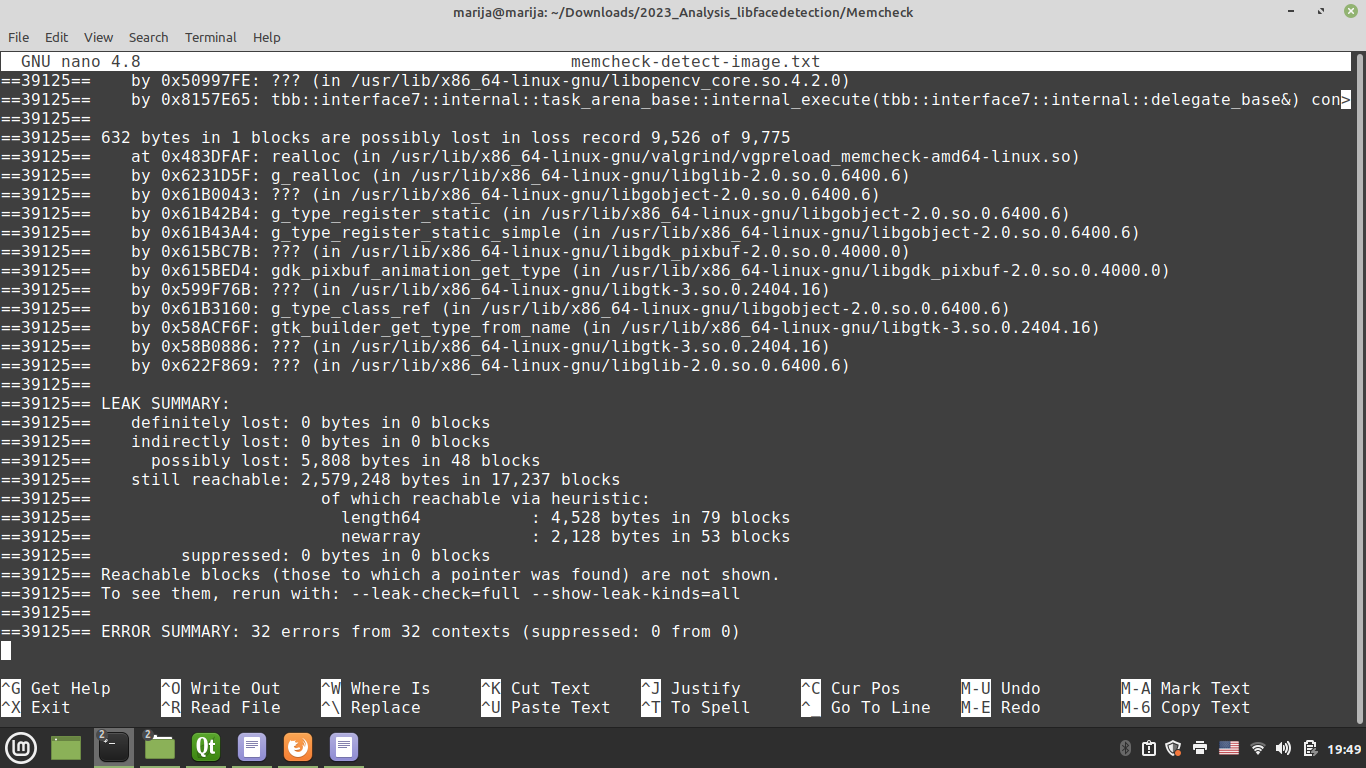
\includegraphics[width=12cm]{img/memcheck/memcheck-detect-image.png}
    \caption{Deo izlaza alata $Memcheck$ nad $detect-image.$}
    \label{di:mcheck}
\end{figure}

\begin{figure}[H]
    \centering
    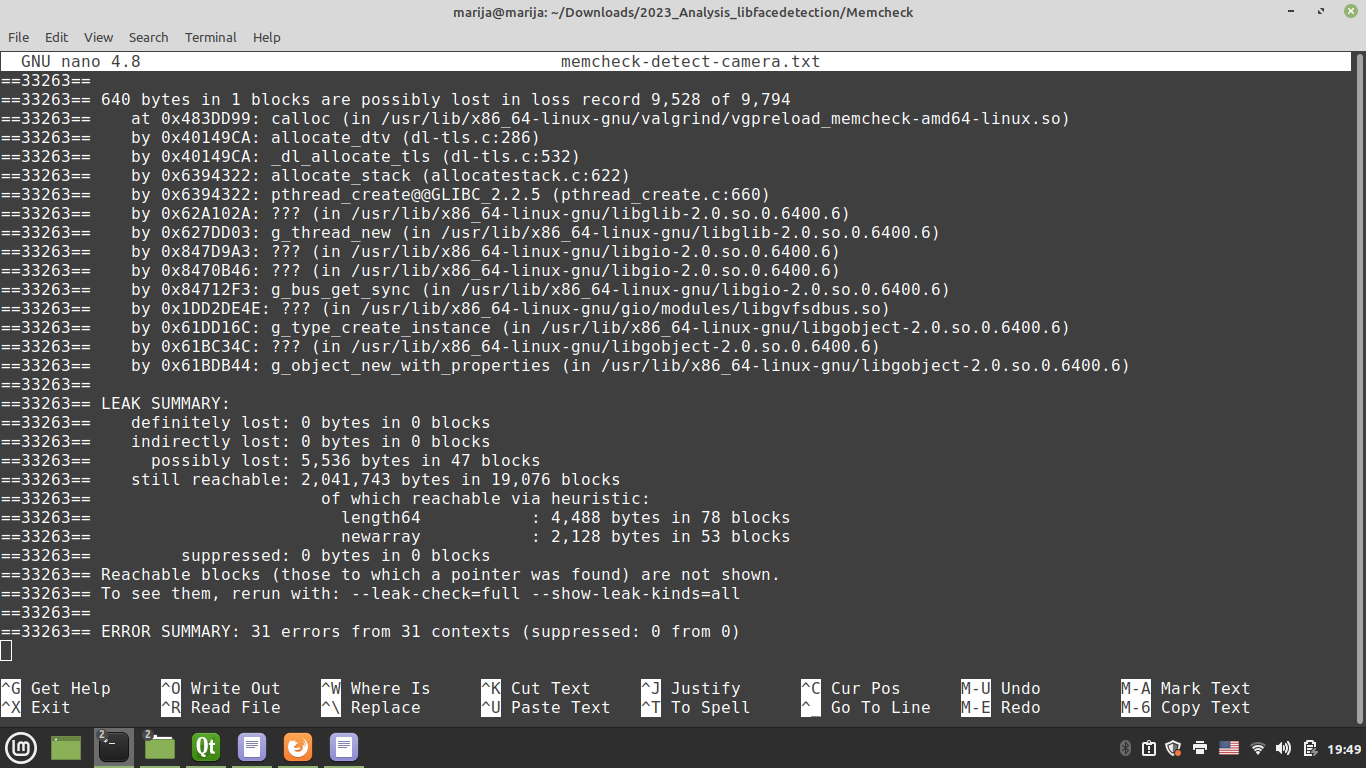
\includegraphics[width=12cm]{img/memcheck/memcheck_detect_camera.png}
    \caption{Deo izlaza alata $Memcheck$ nad $detect-camera.$}
    \label{dc:mcheck}
\end{figure}
\subsubsection{$Massif$}

Za vizuelizaciju rezultata korish\-c1en $massif_visualizer$, koji je preuzet sa \href{https://github.com/KDE/massif-visualizer}{$https://github.com/KDE/massif-visualizer$}, gde se mozhe pronac1i detaljno uputstvo za instaliranje i pokretanje.

\begin{figure}[H]
    \centering
    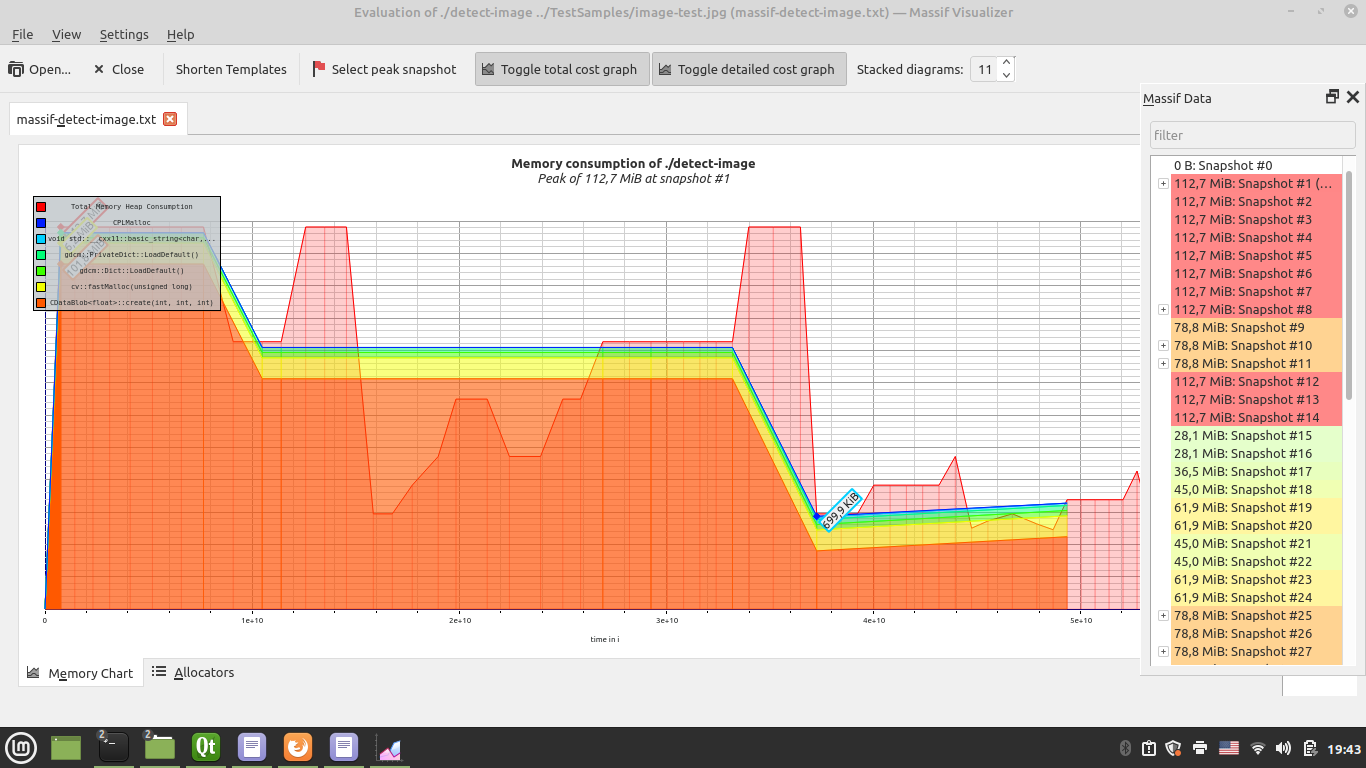
\includegraphics[width=12cm]{img/massif/massif_detect_image_memory.png}
    \caption{}
    \label{dim:massif}
\end{figure}
\begin{figure}[H]
    \centering
    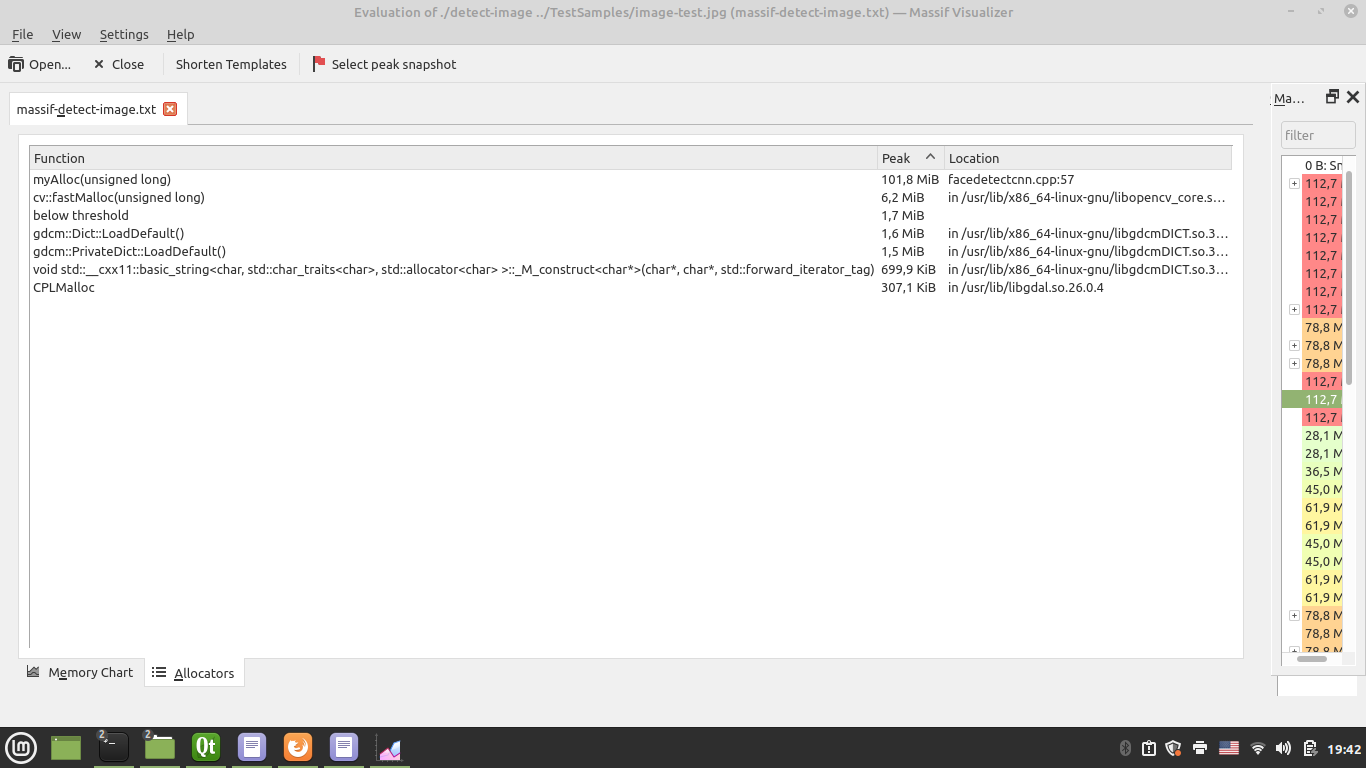
\includegraphics[width=12cm]{img/massif/massif_detect_image_allocators.png}
    \caption{}
    \label{dima:massif}
\end{figure}

\begin{figure}[H]
    \centering
    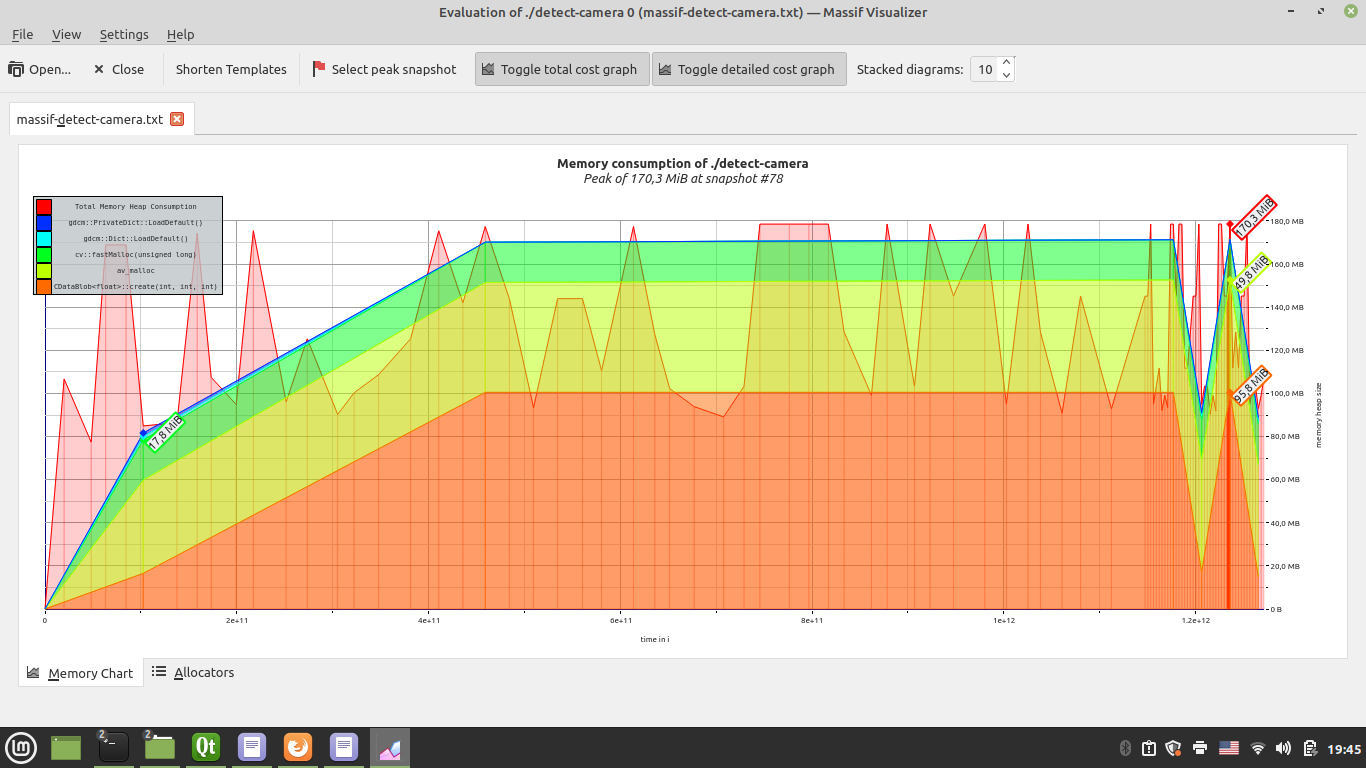
\includegraphics[width=12cm]{img/massif/massif_detect_camera_memory1.png}
    \caption{}
    \label{dcm:massif}
\end{figure}

\begin{figure}[H]
    \centering
    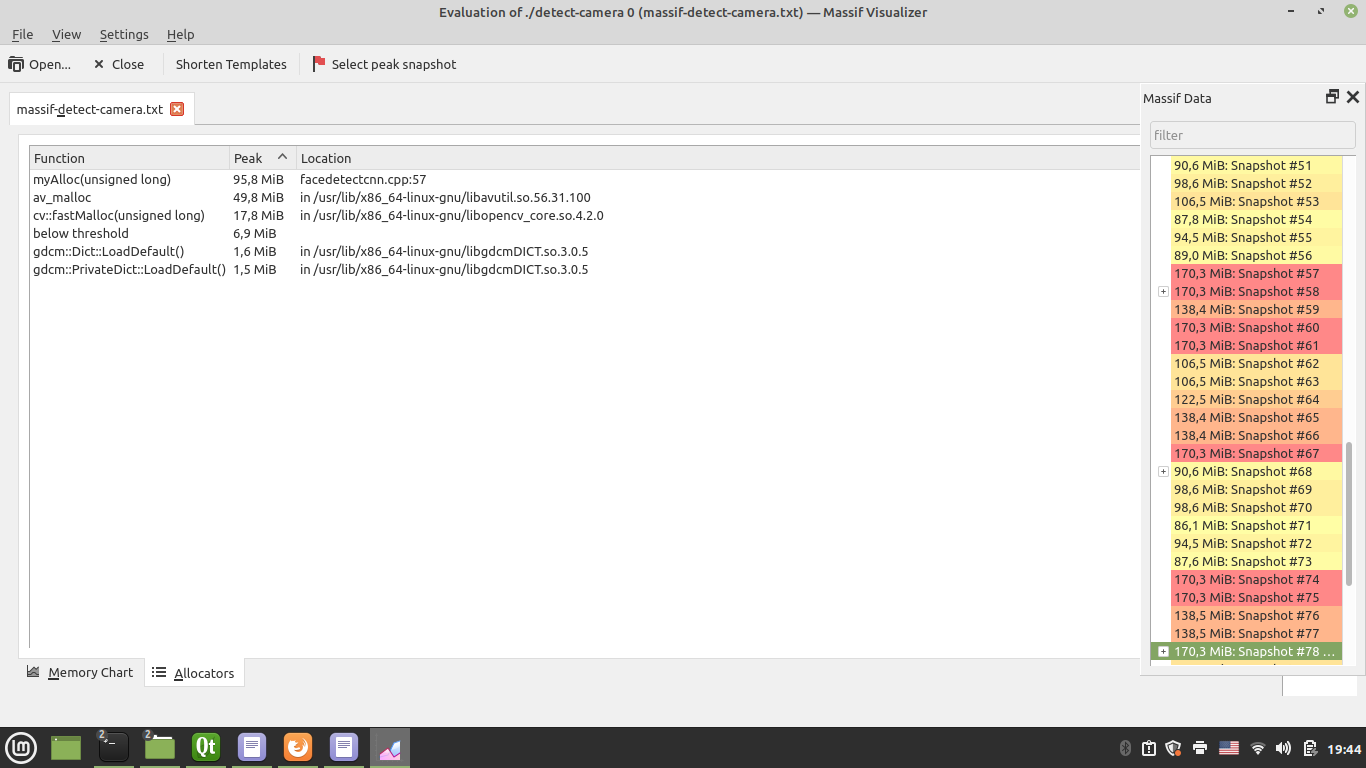
\includegraphics[width=12cm]{img/massif/massif_detect_camera_allocators.png}
    \caption{}
    \label{dcma:massif}
\end{figure}


\subsection{Statichka analiza}
\subsubsection{$CppCheck$}
$CppCheck$ je alat za statichku analizu $C/C++$ koda, koji pruzha jedinstvenu analizu za detekciju greshaka, sa fokusom na nedefinisano ponashanje i sa opasnim konstruktima koda. Analiza dobijena $CppCheck$ nije ni saglasna, niti je potpuna. Dakle, mozhe imati i lazhno pozitivne rezultate, kao i lazhno negativne.
Moguc1e poruke:
\begin{itemize}
    \item Greshka - nedefinisano ponashanje (curenje memorije ili curenje resursa)
    \item Stil - redundantnost, nekorish\-c1ene funkcije/promenljive, potencijalne greshke
    \item Performanse - popravka ovih poruka ne garantuje ubrzanje (jer je statichka analiza u pitanju)
    \item Prenosivost
    \item Konfiguracione informacije
\end{itemize}
\paragraph*{Instaliranje i pokretanje alata:}
Detaljna instalacija 
\href{https://cppcheck.sourceforge.io/}{zvanichnoj stranici.} 
Detaljan opis nachina korish\-c1enja alata se mozhe nac1i u \cite{cppCheckMan}.

Prilikom instalacije na Debian distribuciji:
\fontencoding{T1}\selectfont
\begin{minted}{shell-session}
sudo apt-get install cppcheck
\end{minted}

\fontencoding{OT2}\selectfont
Pokretanje alata $cppcheck$ nad projektom $libfacedetection$: 

\fontencoding{T1}\selectfont
\begin{minted}{shell-session}
cppcheck --enable=all --output-file="cppCheckOut.xml" --xml
--inconclusive libfacedetection/
\end{minted}

\fontencoding{OT2}\selectfont
Dodatni flagovi:\\
$--enable = all$ - pronalazak svi greshaka \\
$--output-file$ - definisanje fajla u koji se upisuje \\
$--xml$ - poruke u $xml$ formatu \\
$--inconclusive$ - neuverljive greshke (potencijalni $false$ $positive$)
\\
U okviru alata je moguc1e napraviti $HTML report$ od izlazne poruke sachuvane u $xml$ formatu. 

\fontencoding{T1}\selectfont
\begin{minted}{shell-session}
cppcheck-htmlreport --report-dir=CppCheckReport --output-file="cppCheckOut.xml" 
\end{minted}

\fontencoding{OT2}\selectfont

Skripta za pokretanje alata se nalazi na $github$; u okviru $README$.

Prikaz pokretanja u alata: \ref{msg:cppcheck}

\begin{figure}[H]
    \centering
    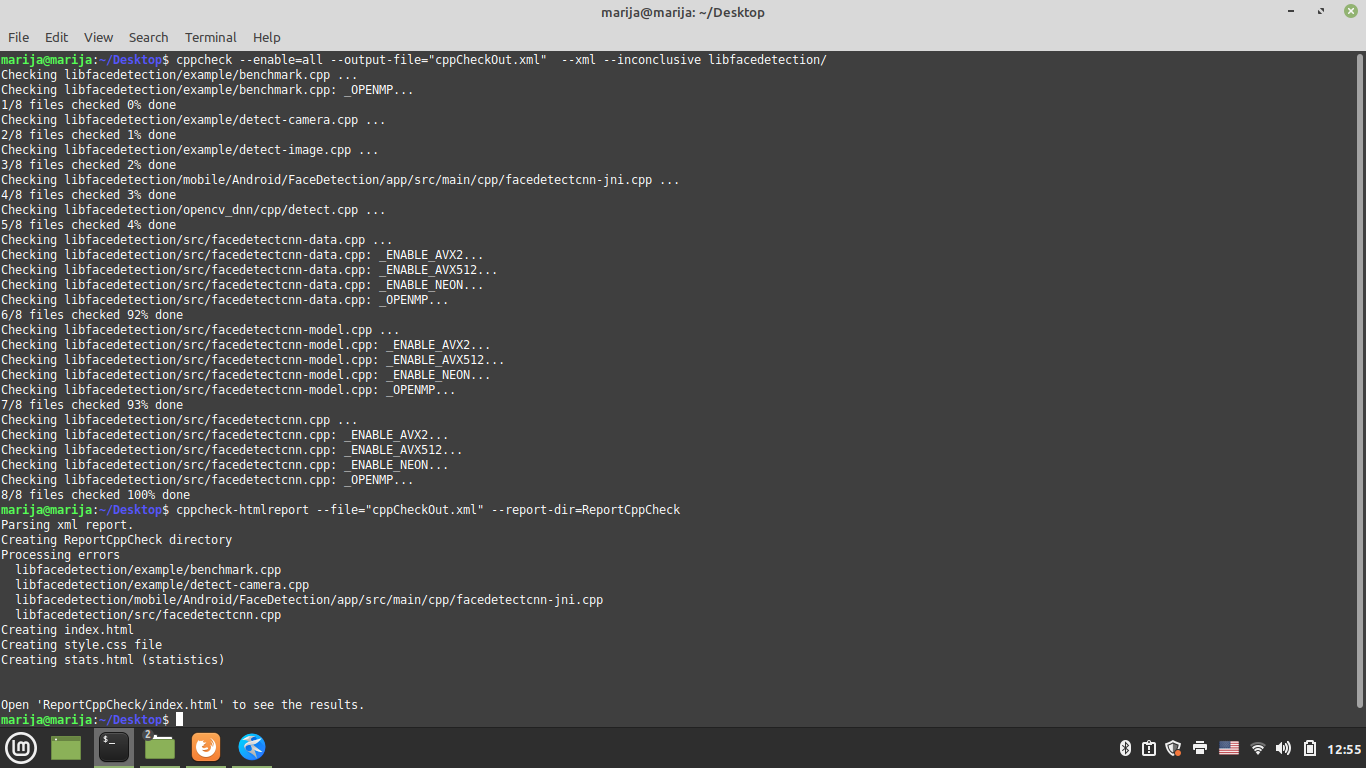
\includegraphics[width=12cm]{img/cppCheck/cppCheckTerminal.png}
    \caption{Poruka o gresh\-ci u $cppCheck$}
    \label{msg:cppcheck}
\end{figure}
%----------------------------------------------------------------%
\paragraph{Rezultati analize:}
Na slici \ref{stats:cppcheck} se nalazi statistika analize.

\begin{figure}[H]
    \centering
    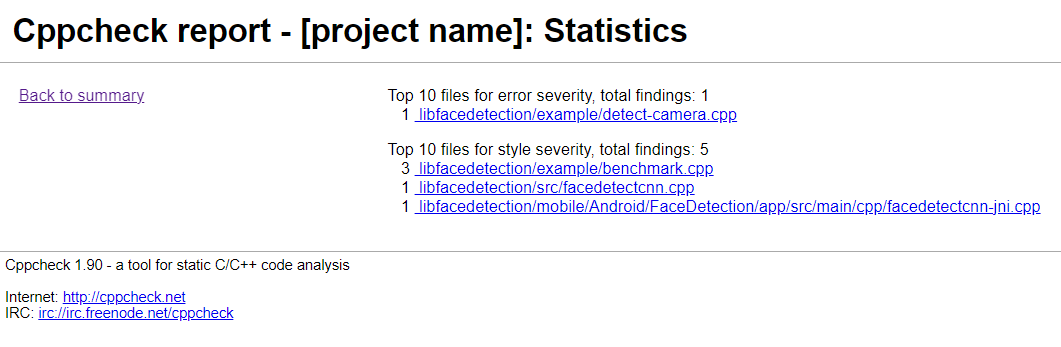
\includegraphics[width=12cm]{img/cppCheck/cppCheckStats.png}
    \caption{Statistika analize alata $cppcheck$}
    \label{stats:cppcheck}
\end{figure}
Na osnovu statistike vidimo da je pronadjena jedna poruka tipa \textit{greshka}, i 5 poruka tipa \textit{stil}.

Detaljnije o porukama se mozhe videti na slici \ref{html:cppcheck}.
\begin{figure}[H]
    \centering
    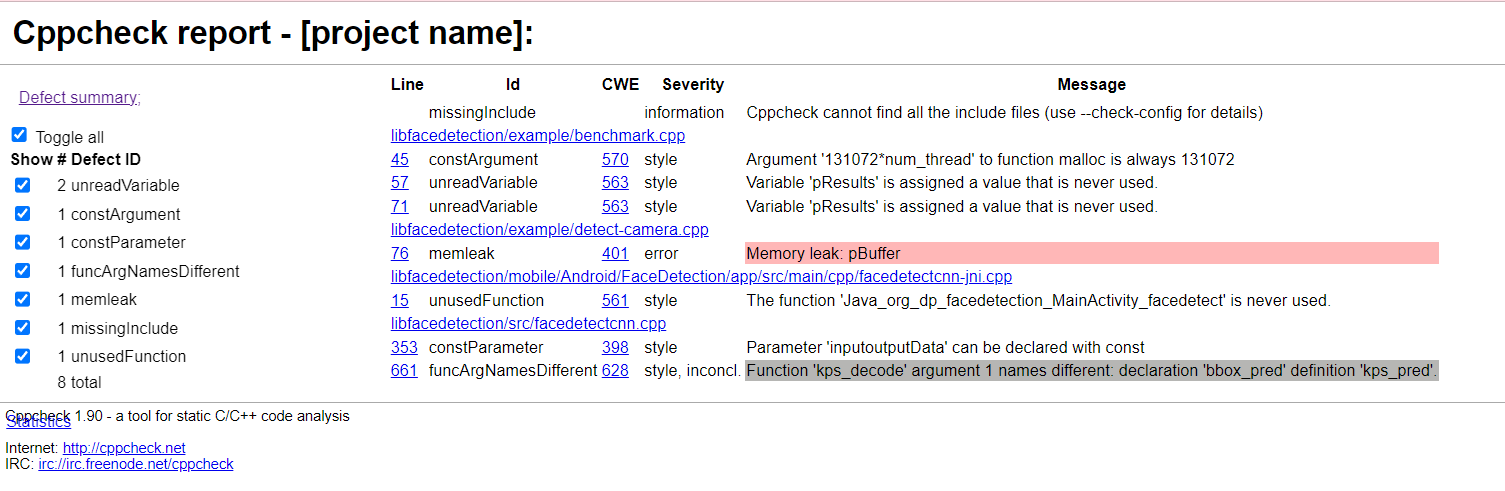
\includegraphics[width=12cm]{img/cppCheck/cppChechHtmlReport.png}
    \caption{Izveshtaj alata $cppcheck$}
    \label{html:cppcheck}
\end{figure}

Greshka se nalazi u 76 liniji u fajlu $detect-camera.cpp$. Deo koda koji izaziva gresku je dat u nastavku:
\fontencoding{T1}\selectfont

\inputminted[frame=lines,
framesep=2mm,
baselinestretch=1.2,
bgcolor=LightGray,
fontsize=\footnotesize,
firstline=55,
lastline=77,
linenos
]{cpp}{detect-camera.cpp}

\fontencoding{OT2}\selectfont
Dakle, memorija koje je alocirana u liniji 59 se ne oslobadja pre prekida izvrshavanja programa, ukoliko je $VideoCapture$ neuspeshno otvoren.

Pored toga su prijavljena upozrorenja za nekorishcene promenljive i funkcije. Detaljan izveshtaj se mozhe pronac1i u okviru repozitorijuma za analizu projekta, u okviru foldera $CppCheckReport.$ U navedenom repozitorijumu je za svaki fajl u kome je alat pronashao neki problem napravljen $html$ izveshtaj sa obelezhenim mestima sa pronadjenim problemima.


\fontencoding{OT2}\selectfont
Takodje, moguc1e je pokretanje alata u okviru razvojnog okrizhenja $QtCreator.$ Poshto nije 
\fontencoding{T1}\selectfont
\textbf{Help->About Plugins -> Code Analyzer}.
\fontencoding{OT2}\selectfont
Izabrati $Cppcheck$. Nakon toga 
je neophodno restartovanje okruzhenje.

Nakon toga: 
\fontencoding{T1}\selectfont
\textbf{Analyze -> Cppcheck}
\fontencoding{OT2}\selectfont
nakon chega se otvara prozor prikazan na slici \ref{qt:cppcheck}.

\begin{figure}[H]
    \centering
    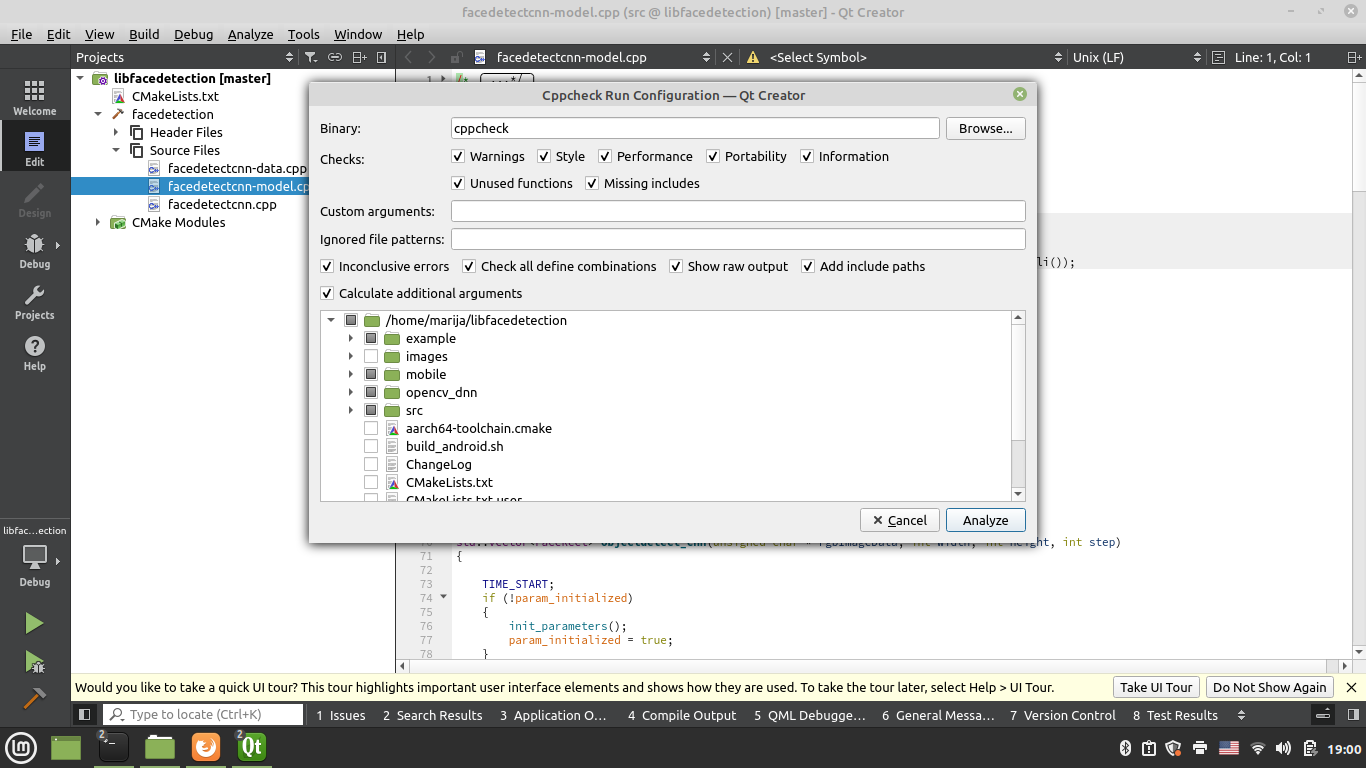
\includegraphics[width=10cm]{img/cppCheck/cppCheckQt.png}
    \caption{Pokretanje alata u okviru $QtCreatora$}
    \label{qt:cppcheck}
\end{figure}

Selektovanjem polja $inconclusive$ $errors$ se prijavljuju i lazhna upozorenja ($false$ $positive$). 

\section{Zakljuchak}

\section{Pokretanje skripti za reprodukovanje rezultata}
\fontencoding{T1}\selectfont


\begin{minted}{shell-session}
git clone https://github.com/MATF-Software-Verification/2023_Analysis_libfacedetection
cd 2023_Analysis_libfacedetection/libfacedetection
git submodule init
git submodule update
\end{minted}

\subsection*{$CppCheck$}
\begin{minted}{shell-session}
cd ../CppCheckReport
bash runCppCheck.sh
\end{minted}

\subsection*{$Prevodjenje biblioteke$}

\begin{minted}{shell-session}
cd libfacedetection
mkdir build
cd build
cmake .. -DCMAKE_INSTALL_PREFIX=install -DBUILD_SHARED_LIBS=ON -DCMAKE_BUILD_TYPE=Release -DDEMO=OFF
cmake --build . --config Release
cmake --build . --config Release --target install
\end{minted}

\subsection*{$Gcov$}
\begin{minted}{shell-session}
cd ../CppCheckReport
bash run_gcov.sh
\end{minted}

\fontencoding{OT2}\selectfont

\bibliographystyle{plain}
\fontencoding{T1}\selectfont
\bibliography{literatura}

\end{document}
